\chapter{Use Case Study}
\label{chap:use-case-study}

\begin{chapterintro}
    % Tady sepsat zakladni info o sekci, ze tu budou vysledky generatoru pro tri zakladni use case
    The following section discusses results for three use cases of full P4 pipeline, including match and action functionality.  
    We provide results of required resources, throughput and number of generated lines, together with required time
    for compilation.
    Using these three use cases, we demonstrate easy extensibility with new protocols and actions.
    Both aspects (extensible set of supported protocols and actions) are important for fast deployment of new 
    applications in these days.
\end{chapterintro}

\section{Test Use Cases}
% Tady vychazet z H2RC2016. Popsat tri zakladni use case studie
% * IPv4 Filter
% * IPv4+IPv6 Filter
% * Full Filter

In this section, we provide three use cases which were selected for demonstration of flexibility and our architecture.
Namely, we will work with following P4-based devices:

\begin{enumerate}
     \item \textbf{IPv4 Filter} is an example of simple engine where the filtering process is based on source IPv4 address. 
     The list of allowed IPv4 addresses and corresponding actions is uploaded at runtime. 
     Two actions are possible: pass or drop the packet. The filter also drops all non-IPv4 traffic by default.    
     \item \textbf{IPv4+IPv6 Filter} extends the IPv4 Filter with further support of IPv6 protocol. All non-IPv4 or non-IPv6 traffic is dropped.
     \item \textbf{Full Filter} extends the IPv4+IPv6 Filter with further support of tagging functionality (VLAN or MPLS). 
     Four actions are possible: pass, drop, VLAN tagging or MPLS tagging. All non-IPv4 or non-IPv6 traffic is dropped.
\end{enumerate}

%Using these three use cases, we demonstrate easy extensibility with new protocols.
%Finally, we extend the IPv4+IPv6 Filter with further tagging functionality which possibly inserts MPLS or VLAN protocol.
%Both aspects, easy extensibility with new protocols and actions, are important for fast deployment of new applications in these
%days.

The following text provides results of required resources, throughput and number of generated lines. 
We selected this views because it allows us to demonstrate the usability and performance of generated architecture 
in real high-speed network environment. The results of proposed use cases are published in 
\cite{2016h2rc-p4,2016MicproP4}.

\section{Experiments}
% V teto kapitole sepsat vysledky, zpusob testovani a vytvorene vysledky.
All introduced use cases were described and translated from P4 language to VHDL using our generator. The generated code was
connected to the NetCOPE \cite{NetCOPEWeb} which is a general platform for rapid development of network applications on 
the family of COMBO cards. The VHDL code was translated for COMBO-100G card \cite{combo-100g} using the Xilinx Vivado 2016.2 design suite. 
The card is capable to process 100\,Gbps and it is equipped with CFP2 transciever cage, PCI-Express generation 3, QDR memory and 
Xilinx Virtex-7 XCVH580T FPGA. 
All use cases were successfully translated with 512 bits wide data bus at frequency of 225.8\,MHz. 
Reached results and further details are provided in following text.

\subsection{Required Resources}
% * pareto grupy ruznych konfiguraci parseru, deparseru
% * grafy pro jednotlive use case + pridat 
% * Tabulka se spotrebovanyma zdrojama na Match+Action pipeline
% * Sepsat postup jak bylo generovano, byla pouzita tato konfigurace

\begin{figure}[b]
    \centering
    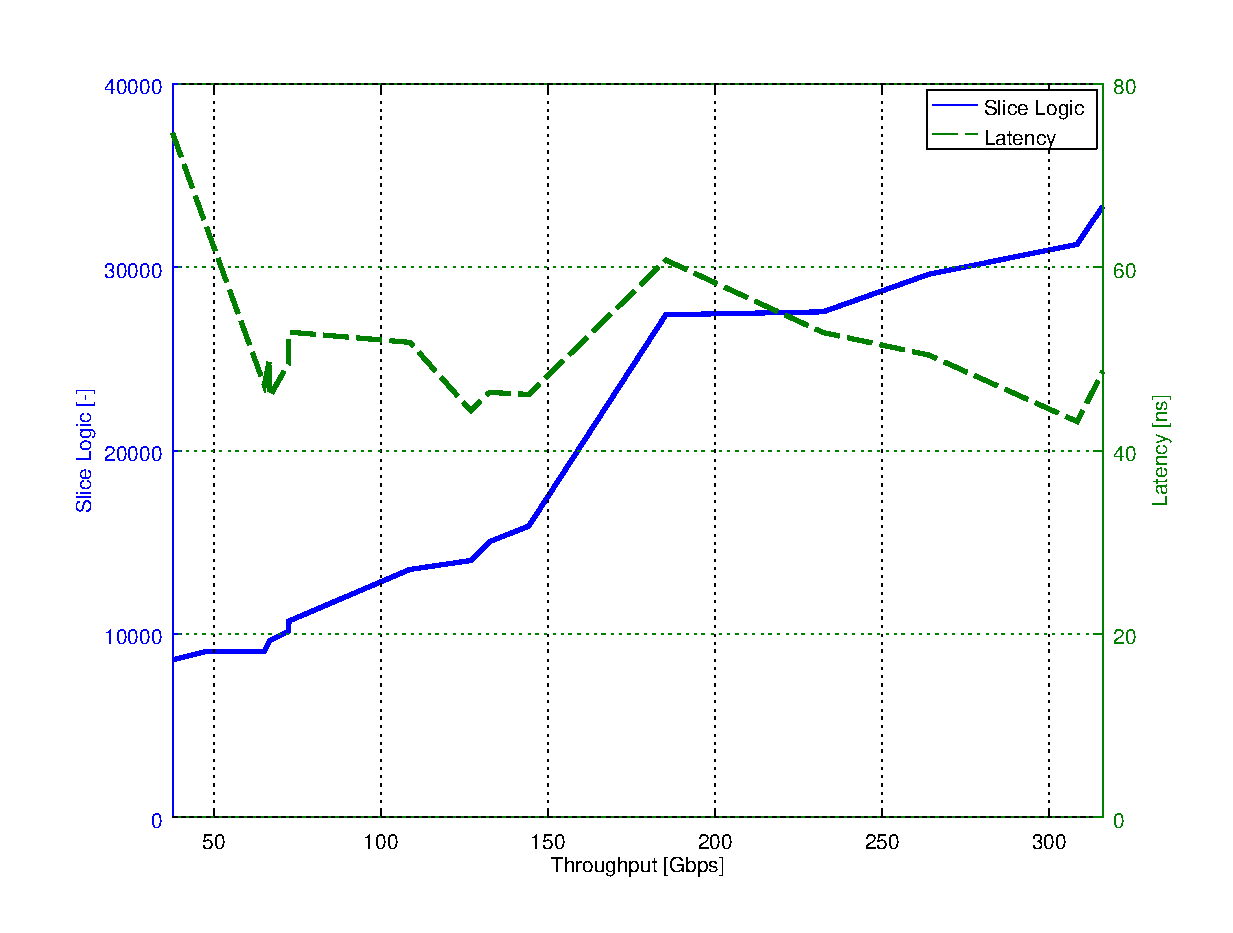
\includegraphics[scale=0.61]{chapters/pic/graphs/p4-pipeline/thr_slice_logic_pareto_ipv4_latency}
    \caption{IPv4 Filter - Pareto optimal solution optimized for throughput and resource utilization with corresponding latency.}
    \label{fig:ipv4ParetoLatency}
\end{figure}

\begin{figure}
    \centering
    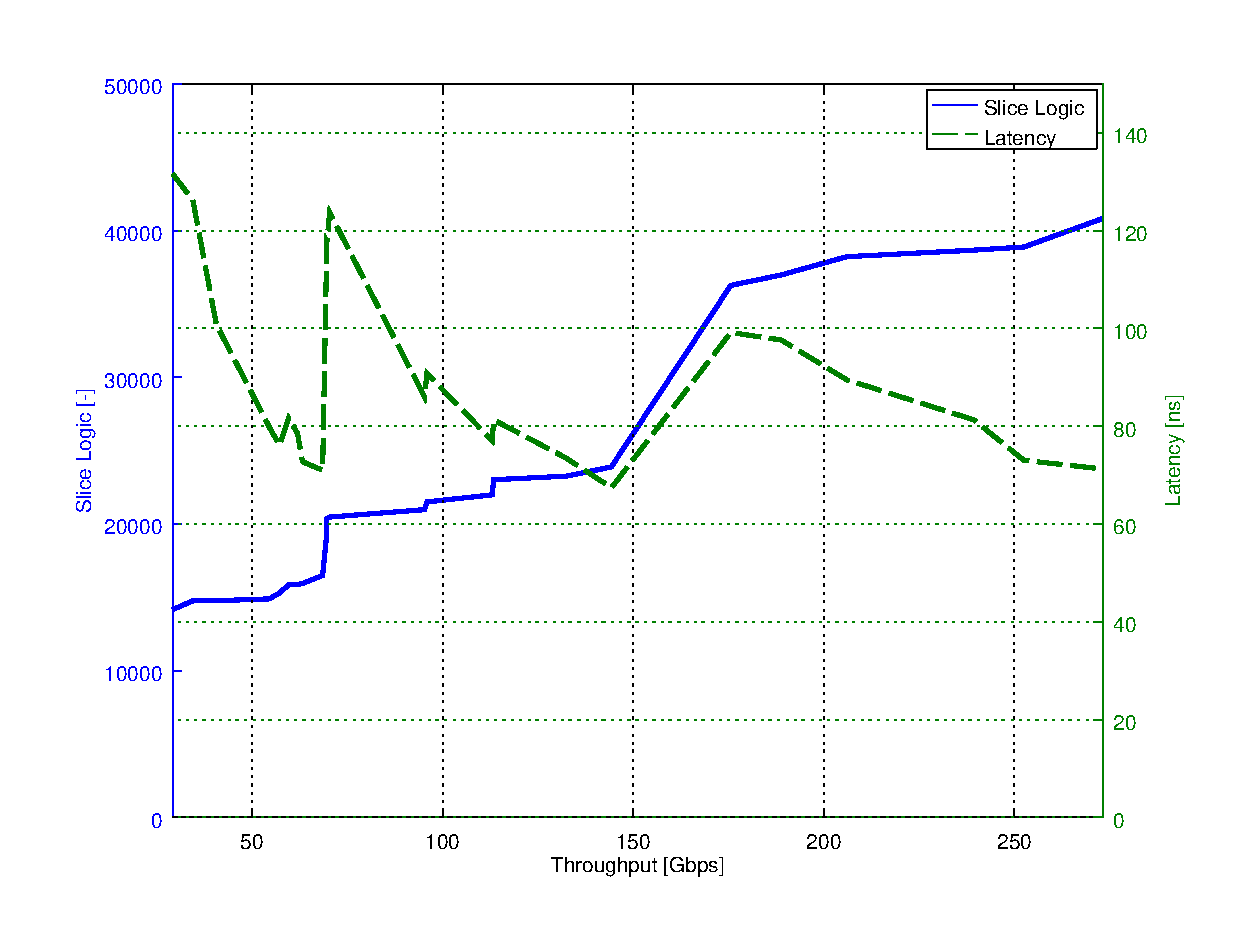
\includegraphics[scale=0.61]{chapters/pic/graphs/p4-pipeline/thr_slice_logic_pareto_ipv46_latency}
    \caption{IPv4+IPv6 Filter - Pareto optimal solution optimized for throughput and resource utilization with corresponding latency.}
    \label{fig:ipv46ParetoLatency}
\end{figure}

\begin{figure}
    \centering
    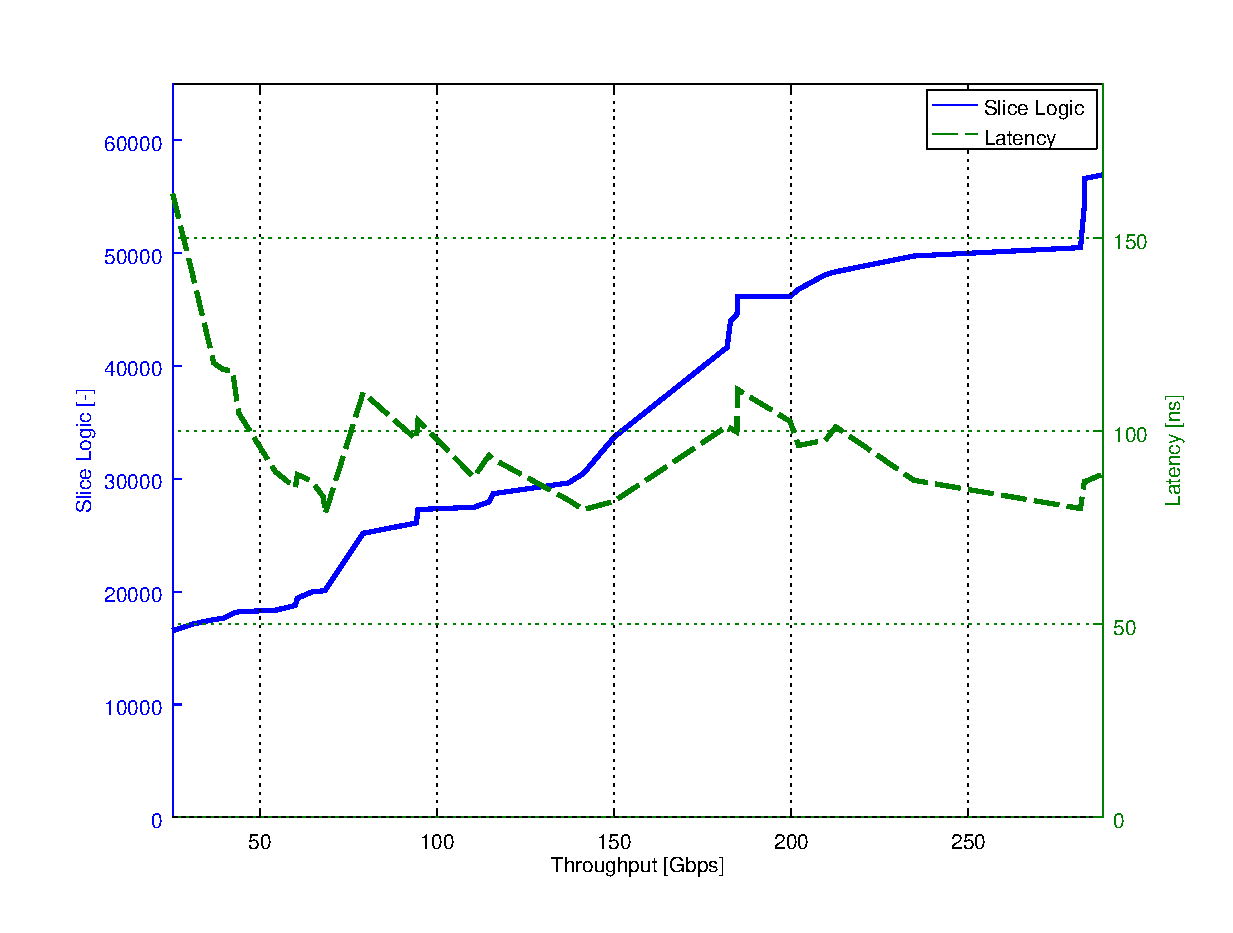
\includegraphics[scale=0.61]{chapters/pic/graphs/p4-pipeline/thr_slice_logic_pareto_full_latency}
    \caption{Full Filter - Pareto optimal solution optimized for throughput and resource utilization with corresponding latency.}
    \label{fig:fullParetoLatency}
\end{figure}

\begin{figure}
    \centering
    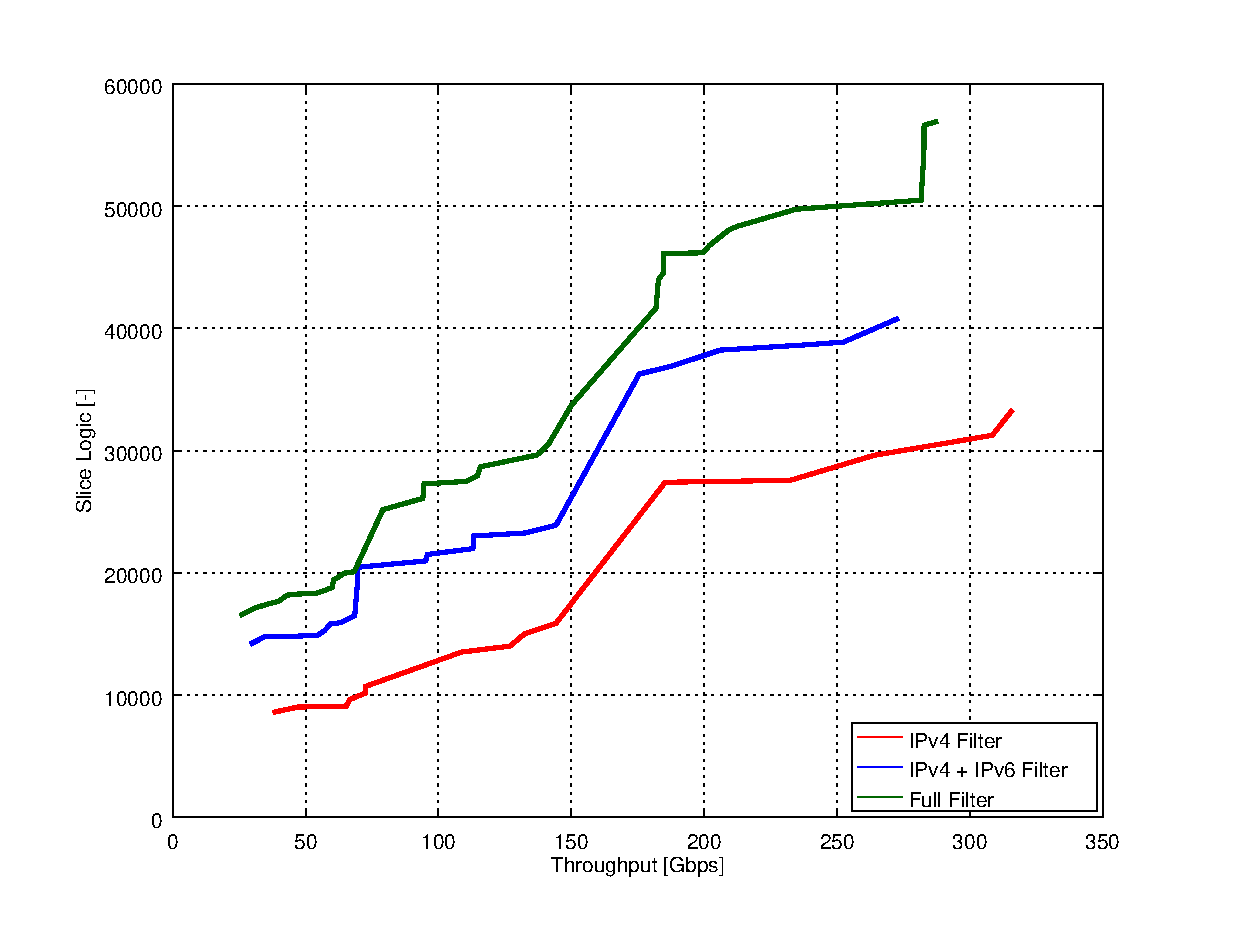
\includegraphics[scale=0.61]{chapters/pic/graphs/p4-pipeline/thr_slice_logic_pareto}
    \caption{Comparison of the FPGA resource utilization versus throughput Pareto sets for tested use cases.}
    \label{fig:useCasesParetoSets}
\end{figure}

In this section, we introduce resource utilization for individual use cases. The resource consumption can be divided into two  
parts --- resources of Match+Action pipeline and resources of parser/deparser.

Resource consumption of Match+Action pipeline is constant because this part of our architecture doesn't have any configurable
pipeline stages. The number of tables, routers, processed packets per one second and required resources after synthesis are shown in
Tab.~\ref{tab:resourcesMatchActionEngines}.
Each Match+Action table was configured to support 32 records in TCAM which is enough for validation of proposed architecture.
We provide required resources of \textit{Search Engines}, including TCAM parts, in Tab.~\ref{tab:resourcesTcamAndSearchEngine}. 
The TCAM part can be replaced by more effective or novel classification approach which leads to different resources.
All results are after synthesis for the Xilinx Virtex-7 XCVH580T FPGA using the Xilinx Vivado 2016.2 design tool. 

The parser/deparser resource utilization is fluctuating because both blocks have 
configurable pipeline modules (i.e., each configuration has different requirements on Slice Logic). 
We developed an automatic testing environment which is capable to translate P4 source, to configure generated VHDL code 
(i.e., the tool setups pipeline stages in parser and deparser), to start the synthesis, and to extract results from the synthesis log. 
This allows us to investigate complex set of possible solutions. 
However, the set of all solutions can be quite large (for complex P4 program) and it can be time consuming to process all 
possible configurations of pipeline stages. 
Due to this, we extend the tool with possibility to select a limited set of configurations which allows us to 
briefly inspect properties of generated devices. The tool was configured to test three different input data widths: 256, 512 and 1024. 
These parameters, data width and configuration of pipeline modules, generate a large space of available solutions.

\begin{table}[t]
    \centering
    \begin{tabular}{|l||c|c||c|c|}
        \hline
        \T \textbf{Project} & \textbf{Tables} & \textbf{Routers} & \textbf{Slice Logic\,[-]} & \textbf{Packet rate\,[Mpps]} \\ \hline\hline
        \T IPv4 Filter      &        2        &        1         &           1917            &             335              \\
        IPv4+IPv6 Filter    &        3        &        2         &           5781            &             339              \\
        Full Filter         &        3        &        2         &           6709            &             318              \\ \hline
    \end{tabular}
    \caption{Required resources of Match+Action engines.}
    \label{tab:resourcesMatchActionEngines}
\end{table}

We provide several graphs: three showing Pareto sets optimized for throughput and chip area without any regard to latency, 
and one for comparison of different Pareto sets of individual use cases. 
Graph of Pareto set for given use cases contains two axes.
The first axis shows required chip area in term of Slice Logic (number of used LUTs plus FlipFlops). 
The second axis shows corresponding latency of those solutions (optimized for throughput and chip area). 
Results of individual use cases are shown in Fig.~\ref{fig:ipv4ParetoLatency}, Fig.~\ref{fig:ipv46ParetoLatency} and 
Fig.~\ref{fig:fullParetoLatency}. It is also important to notice that provided solutions aren't globally optimal because 
our data set doesn't contain all possible solutions. However, the approach with limited configuration set allows to briefly inspect
properties of generated devices in a reasonable time.
Finally, the Fig.~\ref{fig:useCasesParetoSets} introduces comparison of Pareto sets optimized for throughput and chip area 
of provided use cases.

\begin{table}[h]
    \centering
    \begin{tabular}{|l||c|c||c|}
    	\hline
    	\T \textbf{Project} & \textbf{Search Engines\,[-]} & \textbf{BRAM\,[-]} & \textbf{TCAM Engines\,[-]} \\ \hline\hline
    	\T IPv4 Filter      &             956              &         1          &            527             \\
    	IPv4+IPv6 Filter    &             3529             &         1          &            2402            \\
    	Full Filter         &             3907             &         1          &            2406            \\ \hline
    \end{tabular}
    \caption{Resources of Search and TCAM engines; Values are summarized through all tables in given project and they are expressed 
        in term of Slice Logic.}
    \label{tab:resourcesTcamAndSearchEngine}
\end{table}

% Namerene vysledky z Vivado 2016.2
% IPv4 Filter
%================== 
% * IPv4 Filter table
%    + Match Engine --> 551 Lut, 341 Reg, BRAM 1
%    + TCAM --> 418 Lut, 109 Reg 
% * Drop table
%    + Match Engine --> 31 Lut, 33 Reg, BRAM 0
%    + TCAM --> 0 Lut, 0 Reg
%
% IPv4+IPv6 Filter
%==================
% * Drop table
%    + Match Engine --> 28 Lut, 33 Reg, BRAM 0
%    + TCAM --> 0 Lut, 0 Reg
% * Table IPv4 
%    + Match Engine --> 554 Lut, 345 Reg, BRAM 1
%    + TCAM --> 415 Lut, 109 Reg
% * Table IPv6
%    + Match Engine --> 1742 Lut, 827 Reg, BRAM 1
%    + TCAM --> 1577 Lut, 301 Reg
%
% IPv4+IPv6 Tag 
%==================
% * Drop table
%    + Match Engine --> 83 Lut, 34 Reg, BRAM 0
%    + TCAM -->  0 Lut, 0 Reg
% * Table IPv4
%    + Match Engine --> 624 Lut, 438 Reg, BRAM 1
%    + TCAM --> 418 Lut, 109 Reg
% * Tabel IPv6
%    + Match Engine --> 1808 Lut, 920 Reg, BRAM 1
%    + TCAM --> 1578 Lut, 301 Reg

\begin{figure}
    \centering
    \begin{subfigure}[b]{0.8\textwidth}
        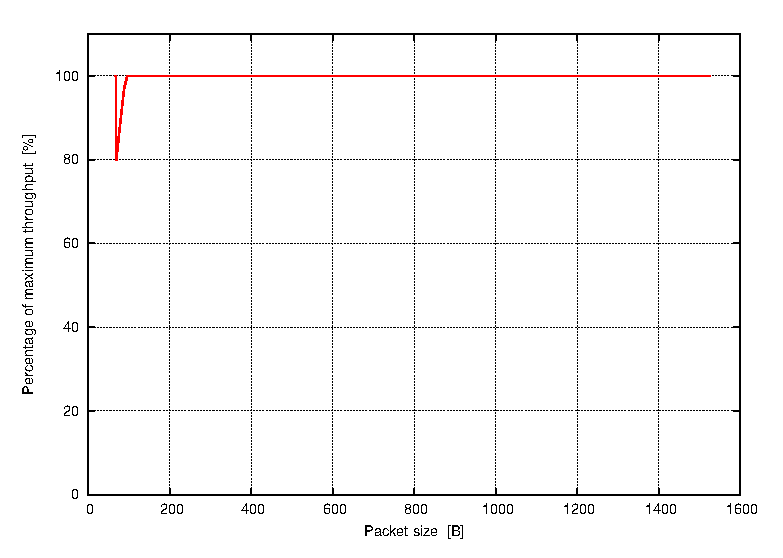
\includegraphics[width=\textwidth]{chapters/pic/graphs/h2rc-cases/ipv46_throughput}
        \caption{Percentage of maximum throughput.}
        \label{fig:bitThroughputIpv46}
    \end{subfigure}
    ~
    \begin{subfigure}[b]{0.8\textwidth}
        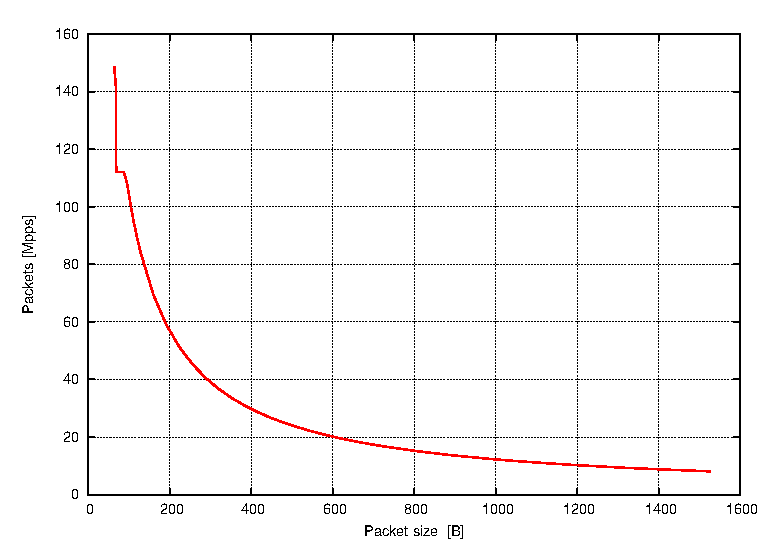
\includegraphics[width=\textwidth]{chapters/pic/graphs/h2rc-cases/ipv46_mpps_throughput}
        \caption{Packet rate.}
        \label{fig:packetThroughputIpv46}
    \end{subfigure}
    
    \caption{Throughput of generated IPv4 and IPv4+IPv6 Filter devices.}
    \label{fig:Ipv46Throughput}
\end{figure}

\begin{figure}
    \centering
    \begin{subfigure}[b]{0.8\textwidth}
        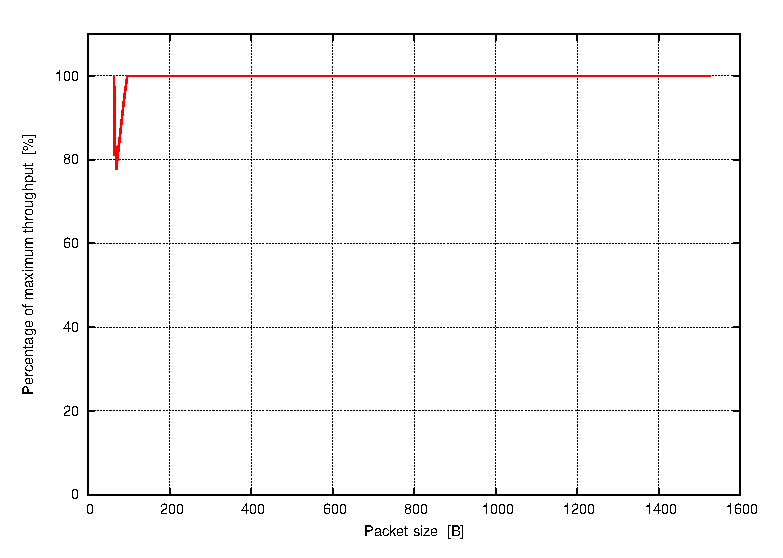
\includegraphics[width=\textwidth]{chapters/pic/graphs/h2rc-cases/full_throughput}
        \caption{Percentage of maximum throughput.}
        \label{fig:bitThroughputFull}
    \end{subfigure}
    ~
    \begin{subfigure}[b]{0.8\textwidth}
        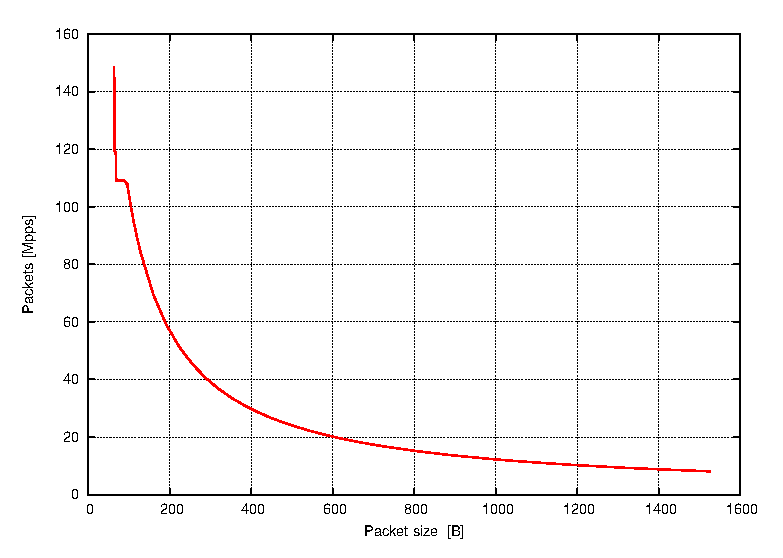
\includegraphics[width=\textwidth]{chapters/pic/graphs/h2rc-cases/full_mpps_throughput}
        \caption{Packet rate.}
        \label{fig:packetThroughputFull}
    \end{subfigure}
    
    \caption{Throughput of generated Full Filter device.}
    \label{fig:FullThroughput}
\end{figure}

\begin{figure}
    \centering
    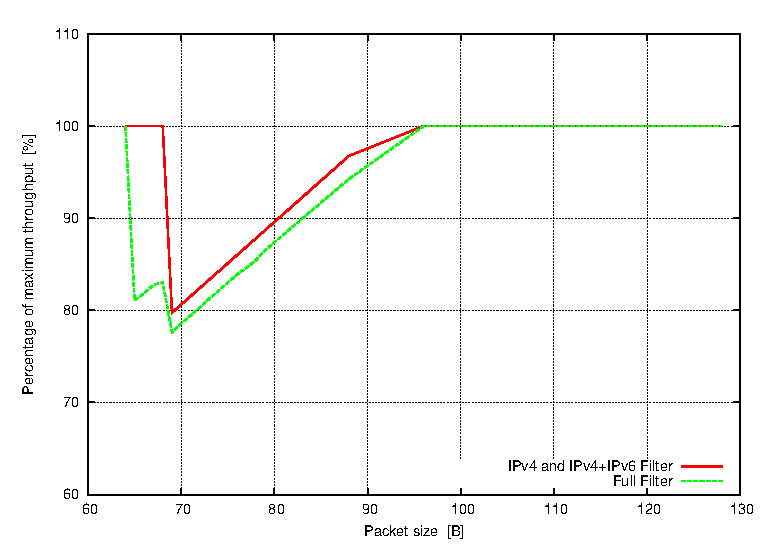
\includegraphics[scale=1.05]{chapters/pic/graphs/h2rc-cases/detail_throughput_ineff}
    \caption{Detail of IPv4, IPv4+IPv6 and Full Filter throughput for small packet sizes.}
    \label{fig:detailThroughputShortPacketLengts}
\end{figure}

\subsection{Throughput}
% * vysledky propustnosti jednotlivych reseni (vuci spirentu), sepsat jednotlive konfigurace ktere se povedly syntetizovat
% ** MPPS + Gbp
%
% Spirent generator byl nakonfigurovan, aby z 19 streamu
% * 6 streamu delal MPLS tag (31%)
% * 6 streamu delal VLAN tag (31%)

We measured throughput of all use cases in high-speed environment. We also created configuration tools capable to upload a user defined rule set.
The rule set was prepared for utilization of each implemented functionality. Therefore, we simulate a situation when 
incoming traffic is distributed across all supported functions. The Fig.~\ref{fig:Ipv46Throughput} shows percentage throughput
of IPv4 and IPv4+IPv6 Filter for generated traffic at speed of 100\,Gbps and a number of processed packets per one second. 
The Fig.~\ref{fig:FullThroughput} introduces the same but for the Full Filter use case.

All tests were performed against Spirent's Hypermetrics MX-100G-F1 module (SPT-N11U chassis).
The proposed results show that our architecture is capable to hit 100\,Gbps. However, there are some 
packet lengths when an inefficiency in deparser causes decrease of throughput. This inefficiency is related to insertion
of protocol header before payload because each Protocol Appender works with aligned data at zero offset. 
Therefore, this optimization leads to less effective usage of data bus (i.e., 64 bytes wide data bus cannot be shared by more packets) 
which leads to decrease of output throughput. 

The Full Filter has smaller throughput than IPv4 or IPv4+IPv6 Filter (compare short packet lengths in
Fig.~\ref{fig:detailThroughputShortPacketLengts}).
This is caused by insertion of four additional bytes (MPLS or VLAN tag) to a packet which leads to decrease of 
input throughput because deparser pipeline needs to be stalled during insertion. 
The Full Filter tags approximately 62\% of incoming traffic (31\% with MPLS tags and 31\% with VLAN tags).

\subsection{Generated Code vs. Total Lines of Code}
% * metrika poctu generovanych casti kodu vs. vsech radku (da se pouzit obsah souboru vivado.prj vs. vygenerovane soubory z p4-vhdl)
In this section, we introduce possible speedup in development of high-speed network devices. 
Reached results for individual use cases are shown in Tab.~\ref{tab:generatedVsTotalLines}.
The table contains compilation times of corresponding P4 source code (number of P4 source code lines is included). 
The \textbf{Generated lines} column expresses effort of the generator. For example, we generated 6283 lines of VHDL code from 91 lines
of P4 source code. The \textbf{Total lines} is a sum of generated lines and lines of library source code (FIFO, TCAM, and so on).
Table also shows that the generator produces approximately one third of each project. The VHDL code is generated from few lines
of P4 source code during two seconds.

% Vsechny casy jsou z prikazu date, real time, testovano na preklad4
% Generated lines (generovane radky v p4vhdl, bez library), Total lines (celkovy pocet radku vcetne knihovnich veci), 2570 radku vhdl_lib veci
\begin{table}[h]
    \centering
    \begin{tabular}{|l||c|c||c|c|}
        \hline
        \T \textbf{Project} & \textbf{P4 lines} & \textbf{Time\,[s]} & \textbf{Generated lines} & \textbf{Total lines} \\ \hline\hline
        \T IPv4 Filter      &        91         &       1.574        &           6283           &        24791         \\
        IPv4+IPv6 Filter    &        129        &       1.818        &           9888           &        28396         \\
        Full Filter         &        212        &       1.929        &          13824           &        32332         \\ \hline
    \end{tabular}
    \caption{Generated code versus total lines of code.}
    \label{tab:generatedVsTotalLines}
\end{table}

\section{Summary}
This chapter provides results of our architecture which was generated from abstract description in P4 language. 
The text introduces three use cases --- IPv4 Filter, IPv4+IPv6 Filter and Full Filter. 
These use cases demonstrate the flexibility and easy extensibility with support of new protocols and actions. 
All devices were generated in two seconds from
several lines of P4 source. This makes the development more effective. For example, developer can be focused on implementation of novel
hardware approaches related to classification because new module can be connected to the existing infrastructure. 
Text also provides Pareto sets optimized for throughput and resource requirements of individual use cases. 
Finally, all use cases were synthesized for COMBO-100G card and tested against Spirent network test device. 
Each use case is capable to hit throughput of 100\,Gbps at frequency of 225.8\,MHz on Xilinx Virtex-7 XCVH580T FPGA.
The results from this chapter are published in \cite{2016h2rc-p4,2016MicproP4}.